\documentclass{standalone}
\usepackage{pgfplots}
\pgfplotsset{compat=1.18}
\usepgfplotslibrary{fillbetween}

\begin{document}
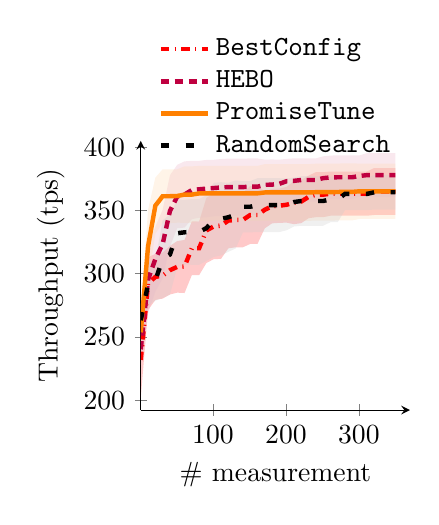
\begin{tikzpicture}
    \begin{axis}[
      axis x line  = bottom,
      axis y line  = left,
      width=5cm, height=5cm, 
      xlabel={\# measurement},
      ylabel={Throughput (tps)},
      xmin=1.0000, xmax=370.0000,
      ymin=192.1300, ymax=405.1052,
      legend cell align=left,
      legend columns=1,
      legend style={
        draw=none, fill=none,
        at={(0.98,0.9)}, anchor=south east,
        legend cell align=left
      }
    ]


\addplot[
    red,
    dashdotted,
    ultra thick, forget plot
] coordinates {
(1.0000, 231.8410) (11.0000, 292.2210) (21.0000, 297.4840) (31.0000, 298.5560) (41.0000, 302.7970) (51.0000, 305.4540) (61.0000, 305.7280) (71.0000, 320.1620) (81.0000, 320.1620) (91.0000, 334.3080) (101.0000, 337.4150) (111.0000, 338.0640) (121.0000, 342.0340) (131.0000, 342.6340) (141.0000, 342.6340) (151.0000, 346.4560) (161.0000, 346.4560) (171.0000, 350.6290) (181.0000, 353.4570) (191.0000, 353.8230) (201.0000, 354.5860) (211.0000, 356.3080) (221.0000, 357.1390) (231.0000, 360.7920) (241.0000, 362.5310) (251.0000, 362.5310) (261.0000, 363.4030) (271.0000, 363.4030) (281.0000, 363.4030) (291.0000, 363.4030) (301.0000, 363.4030) (311.0000, 363.4030) (321.0000, 365.0620) (331.0000, 365.0620) (341.0000, 365.0620) (350.0000, 365.0620)
}; 
\addlegendentry{\texttt{BestConfig}}

\addplot[
name path=upper0,
draw=none, forget plot
] coordinates {
(1.0000, 261.8713) (11.0000, 313.1449) (21.0000, 315.6845) (31.0000, 316.7752) (41.0000, 322.0210) (51.0000, 325.8844) (61.0000, 326.7054) (71.0000, 341.4213) (81.0000, 341.4213) (91.0000, 360.1366) (101.0000, 363.3199) (111.0000, 364.3603) (121.0000, 363.9696) (131.0000, 364.3403) (141.0000, 364.3403) (151.0000, 369.3578) (161.0000, 369.3578) (171.0000, 365.2764) (181.0000, 367.0379) (191.0000, 367.3728) (201.0000, 368.7579) (211.0000, 373.4075) (221.0000, 374.2133) (231.0000, 377.6531) (241.0000, 380.3435) (251.0000, 380.3435) (261.0000, 380.8934) (271.0000, 380.8934) (281.0000, 380.8934) (291.0000, 380.8934) (301.0000, 380.8934) (311.0000, 380.8934) (321.0000, 383.6392) (331.0000, 383.6392) (341.0000, 383.6392) (350.0000, 383.6392)
}; 

\addplot[
name path=lower0,
draw=none, forget plot
] coordinates {
(1.0000, 201.8107) (11.0000, 271.2971) (21.0000, 279.2835) (31.0000, 280.3368) (41.0000, 283.5730) (51.0000, 285.0236) (61.0000, 284.7506) (71.0000, 298.9027) (81.0000, 298.9027) (91.0000, 308.4794) (101.0000, 311.5101) (111.0000, 311.7677) (121.0000, 320.0984) (131.0000, 320.9277) (141.0000, 320.9277) (151.0000, 323.5542) (161.0000, 323.5542) (171.0000, 335.9816) (181.0000, 339.8761) (191.0000, 340.2732) (201.0000, 340.4141) (211.0000, 339.2085) (221.0000, 340.0647) (231.0000, 343.9309) (241.0000, 344.7185) (251.0000, 344.7185) (261.0000, 345.9126) (271.0000, 345.9126) (281.0000, 345.9126) (291.0000, 345.9126) (301.0000, 345.9126) (311.0000, 345.9126) (321.0000, 346.4848) (331.0000, 346.4848) (341.0000, 346.4848) (350.0000, 346.4848)
}; 

% ========= file shading =========
\addplot[
    red!70,
    fill opacity=0.30, forget plot
] fill between[
    of=upper0 and lower0,
];


\addplot[
    purple,
    densely dashed,
    ultra thick, forget plot
] coordinates {
(1.0000, 240.1760) (11.0000, 295.3720) (21.0000, 311.6410) (31.0000, 323.4420) (41.0000, 349.6870) (51.0000, 361.0960) (61.0000, 362.7180) (71.0000, 366.2390) (81.0000, 366.8140) (91.0000, 367.3550) (101.0000, 367.8130) (111.0000, 368.2460) (121.0000, 368.5550) (131.0000, 368.5550) (141.0000, 368.5550) (151.0000, 368.8790) (161.0000, 368.8790) (171.0000, 370.3590) (181.0000, 370.5080) (191.0000, 371.1650) (201.0000, 373.2150) (211.0000, 373.5080) (221.0000, 374.1640) (231.0000, 374.1640) (241.0000, 374.1640) (251.0000, 375.6350) (261.0000, 376.2260) (271.0000, 376.3310) (281.0000, 376.3710) (291.0000, 376.3710) (301.0000, 377.3670) (311.0000, 378.0270) (321.0000, 378.0270) (331.0000, 378.0270) (341.0000, 378.0270) (350.0000, 378.0270)
}; 
\addlegendentry{\texttt{HEBO}}

\addplot[
name path=upper1,
draw=none, forget plot
] coordinates {
(1.0000, 252.4085) (11.0000, 322.2653) (21.0000, 337.2947) (31.0000, 350.5685) (41.0000, 377.8667) (51.0000, 386.1928) (61.0000, 388.9255) (71.0000, 389.3293) (81.0000, 389.3509) (91.0000, 390.0583) (101.0000, 390.1666) (111.0000, 390.7598) (121.0000, 391.1247) (131.0000, 391.1247) (141.0000, 391.1247) (151.0000, 391.2213) (161.0000, 391.2213) (171.0000, 390.3002) (181.0000, 390.4322) (191.0000, 390.2884) (201.0000, 390.8911) (211.0000, 391.3049) (221.0000, 391.2890) (231.0000, 391.2890) (241.0000, 391.2890) (251.0000, 392.9058) (261.0000, 393.4887) (271.0000, 393.6932) (281.0000, 393.6835) (291.0000, 393.6835) (301.0000, 393.6838) (311.0000, 395.4245) (321.0000, 395.4245) (331.0000, 395.4245) (341.0000, 395.4245) (350.0000, 395.4245)
}; 

\addplot[
name path=lower1,
draw=none, forget plot
] coordinates {
(1.0000, 227.9435) (11.0000, 268.4787) (21.0000, 285.9873) (31.0000, 296.3155) (41.0000, 321.5073) (51.0000, 335.9992) (61.0000, 336.5105) (71.0000, 343.1487) (81.0000, 344.2771) (91.0000, 344.6517) (101.0000, 345.4594) (111.0000, 345.7322) (121.0000, 345.9853) (131.0000, 345.9853) (141.0000, 345.9853) (151.0000, 346.5367) (161.0000, 346.5367) (171.0000, 350.4178) (181.0000, 350.5838) (191.0000, 352.0416) (201.0000, 355.5389) (211.0000, 355.7111) (221.0000, 357.0390) (231.0000, 357.0390) (241.0000, 357.0390) (251.0000, 358.3642) (261.0000, 358.9633) (271.0000, 358.9688) (281.0000, 359.0585) (291.0000, 359.0585) (301.0000, 361.0502) (311.0000, 360.6295) (321.0000, 360.6295) (331.0000, 360.6295) (341.0000, 360.6295) (350.0000, 360.6295)
}; 

% ========= file shading =========
\addplot[
    purple!30,
    fill opacity=0.30, forget plot
] fill between[
    of=upper1 and lower1,
];


\addplot[
    orange,
    solid,
    ultra thick, forget plot
] coordinates {
(1.0000, 253.6100) (11.0000, 321.7610) (21.0000, 353.8880) (31.0000, 361.3420) (41.0000, 361.3420) (51.0000, 361.5200) (61.0000, 362.6310) (71.0000, 362.6310) (81.0000, 363.5630) (91.0000, 363.6000) (101.0000, 363.6000) (111.0000, 363.6000) (121.0000, 363.6000) (131.0000, 363.6000) (141.0000, 363.6000) (151.0000, 363.6000) (161.0000, 363.6000) (171.0000, 364.3130) (181.0000, 364.3130) (191.0000, 364.3130) (201.0000, 364.3130) (211.0000, 364.3130) (221.0000, 364.3130) (231.0000, 364.3130) (241.0000, 364.5320) (251.0000, 364.5320) (261.0000, 364.5320) (271.0000, 364.6900) (281.0000, 364.7740) (291.0000, 364.7800) (301.0000, 365.2350) (311.0000, 365.2350) (321.0000, 365.2350) (331.0000, 365.2350) (341.0000, 365.2350) (350.0000, 365.2350)
}; 
\addlegendentry{\texttt{PromiseTune}}

\addplot[
name path=upper2,
draw=none, forget plot
] coordinates {
(1.0000, 268.7419) (11.0000, 350.6650) (21.0000, 376.0959) (31.0000, 382.6303) (41.0000, 382.6303) (51.0000, 382.6638) (61.0000, 384.9611) (71.0000, 384.9611) (81.0000, 385.3293) (91.0000, 385.3124) (101.0000, 385.3124) (111.0000, 385.3124) (121.0000, 385.3124) (131.0000, 385.3124) (141.0000, 385.3124) (151.0000, 385.3124) (161.0000, 385.3124) (171.0000, 386.7311) (181.0000, 386.7311) (191.0000, 386.7311) (201.0000, 386.7311) (211.0000, 386.7311) (221.0000, 386.7311) (231.0000, 386.7311) (241.0000, 387.0764) (251.0000, 387.0764) (261.0000, 387.0764) (271.0000, 387.1684) (281.0000, 387.3247) (291.0000, 387.3220) (301.0000, 387.1517) (311.0000, 387.1517) (321.0000, 387.1517) (331.0000, 387.1517) (341.0000, 387.1517) (350.0000, 387.1517)
}; 

\addplot[
name path=lower2,
draw=none, forget plot
] coordinates {
(1.0000, 238.4781) (11.0000, 292.8570) (21.0000, 331.6801) (31.0000, 340.0537) (41.0000, 340.0537) (51.0000, 340.3762) (61.0000, 340.3009) (71.0000, 340.3009) (81.0000, 341.7967) (91.0000, 341.8876) (101.0000, 341.8876) (111.0000, 341.8876) (121.0000, 341.8876) (131.0000, 341.8876) (141.0000, 341.8876) (151.0000, 341.8876) (161.0000, 341.8876) (171.0000, 341.8949) (181.0000, 341.8949) (191.0000, 341.8949) (201.0000, 341.8949) (211.0000, 341.8949) (221.0000, 341.8949) (231.0000, 341.8949) (241.0000, 341.9876) (251.0000, 341.9876) (261.0000, 341.9876) (271.0000, 342.2116) (281.0000, 342.2233) (291.0000, 342.2380) (301.0000, 343.3183) (311.0000, 343.3183) (321.0000, 343.3183) (331.0000, 343.3183) (341.0000, 343.3183) (350.0000, 343.3183)
}; 

% ========= file shading =========
\addplot[
    orange!30,
    fill opacity=0.30, forget plot
] fill between[
    of=upper2 and lower2,
];


\addplot[
    black,
    loosely dashed,
    ultra thick, forget plot
] coordinates {
(1.0000, 263.1770) (11.0000, 291.8320) (21.0000, 294.7770) (31.0000, 311.5460) (41.0000, 315.2240) (51.0000, 332.0600) (61.0000, 332.7900) (71.0000, 333.0970) (81.0000, 333.0970) (91.0000, 336.1120) (101.0000, 342.6550) (111.0000, 343.4820) (121.0000, 344.6670) (131.0000, 346.8650) (141.0000, 352.9980) (151.0000, 352.9980) (161.0000, 354.2680) (171.0000, 354.2680) (181.0000, 354.2680) (191.0000, 354.2680) (201.0000, 354.8910) (211.0000, 356.7420) (221.0000, 357.5560) (231.0000, 357.5560) (241.0000, 357.5560) (251.0000, 357.5560) (261.0000, 358.8370) (271.0000, 358.8370) (281.0000, 363.1740) (291.0000, 363.1740) (301.0000, 363.1740) (311.0000, 363.1740) (321.0000, 364.4560) (331.0000, 364.4560) (341.0000, 364.4560) (350.0000, 364.4560)
}; 
\addlegendentry{\texttt{RandomSearch}}

\addplot[
name path=upper3,
draw=none, forget plot
] coordinates {
(1.0000, 280.9611) (11.0000, 308.9844) (21.0000, 310.9465) (31.0000, 342.2059) (41.0000, 346.9628) (51.0000, 358.6958) (61.0000, 358.4133) (71.0000, 359.0847) (81.0000, 359.0847) (91.0000, 362.0485) (101.0000, 371.9628) (111.0000, 372.4334) (121.0000, 371.9941) (131.0000, 373.7563) (141.0000, 373.2330) (151.0000, 373.2330) (161.0000, 375.5812) (171.0000, 375.5812) (181.0000, 375.5812) (191.0000, 375.5812) (201.0000, 375.3510) (211.0000, 376.0944) (221.0000, 377.1446) (231.0000, 377.1446) (241.0000, 377.1446) (251.0000, 377.1446) (261.0000, 376.8801) (271.0000, 376.8801) (281.0000, 376.0361) (291.0000, 376.0361) (301.0000, 376.0361) (311.0000, 376.0361) (321.0000, 378.1208) (331.0000, 378.1208) (341.0000, 378.1208) (350.0000, 378.1208)
}; 

\addplot[
name path=lower3,
draw=none, forget plot
] coordinates {
(1.0000, 245.3929) (11.0000, 274.6796) (21.0000, 278.6075) (31.0000, 280.8861) (41.0000, 283.4852) (51.0000, 305.4242) (61.0000, 307.1667) (71.0000, 307.1093) (81.0000, 307.1093) (91.0000, 310.1755) (101.0000, 313.3472) (111.0000, 314.5306) (121.0000, 317.3399) (131.0000, 319.9737) (141.0000, 332.7630) (151.0000, 332.7630) (161.0000, 332.9548) (171.0000, 332.9548) (181.0000, 332.9548) (191.0000, 332.9548) (201.0000, 334.4310) (211.0000, 337.3896) (221.0000, 337.9674) (231.0000, 337.9674) (241.0000, 337.9674) (251.0000, 337.9674) (261.0000, 340.7939) (271.0000, 340.7939) (281.0000, 350.3119) (291.0000, 350.3119) (301.0000, 350.3119) (311.0000, 350.3119) (321.0000, 350.7912) (331.0000, 350.7912) (341.0000, 350.7912) (350.0000, 350.7912)
}; 

% ========= file shading =========
\addplot[
    black!20,
    fill opacity=0.30, forget plot
] fill between[
    of=upper3 and lower3,
];


\addlegendimage{red, dashdotted, ultra thick}
\addlegendentry{\texttt{BestConfig}}
\addlegendimage{purple, densely dashed, ultra thick}
\addlegendentry{\texttt{HEBO}}
\addlegendimage{orange, solid, ultra thick}
\addlegendentry{\texttt{PromiseTune}}
\addlegendimage{black, loosely dashed, ultra thick}
\addlegendentry{\texttt{RandomSearch}}

\end{axis}
\end{tikzpicture}
\end{document}
